\UseRawInputEncoding
\documentclass[12pt,letterpaper]{article}
\usepackage{graphicx,textcomp}
\usepackage{natbib}
\usepackage{setspace}
\usepackage{fullpage}
\usepackage{color}
\usepackage[reqno]{amsmath}
\usepackage{amsthm}
\usepackage{fancyvrb}
\usepackage{amssymb,enumerate}
\usepackage[all]{xy}
\usepackage{endnotes}
\usepackage{lscape}
\newtheorem{com}{Comment}
\usepackage{float}
\usepackage{hyperref}
\newtheorem{lem} {Lemma}
\newtheorem{prop}{Proposition}
\newtheorem{thm}{Theorem}
\newtheorem{defn}{Definition}
\newtheorem{cor}{Corollary}
\newtheorem{obs}{Observation}
\usepackage[compact]{titlesec}
\usepackage{dcolumn}
\usepackage{tikz}
\usetikzlibrary{arrows}
\usepackage{multirow}
\usepackage{xcolor}
\newcolumntype{.}{D{.}{.}{-1}}
\newcolumntype{d}[1]{D{.}{.}{#1}}
\definecolor{light-gray}{gray}{0.65}
\usepackage{url}
\usepackage{listings}
\usepackage{color}

\definecolor{codegreen}{rgb}{0,0.6,0}
\definecolor{codegray}{rgb}{0.5,0.5,0.5}
\definecolor{codepurple}{rgb}{0.58,0,0.82}
\definecolor{backcolour}{rgb}{0.95,0.95,0.92}

\lstdefinestyle{mystyle}{
	backgroundcolor=\color{backcolour},   
	commentstyle=\color{codegreen},
	keywordstyle=\color{magenta},
	numberstyle=\tiny\color{codegray},
	stringstyle=\color{codepurple},
	basicstyle=\footnotesize,
	breakatwhitespace=false,         
	breaklines=true,                 
	captionpos=b,                    
	keepspaces=true,                 
	numbers=left,                    
	numbersep=5pt,                  
	showspaces=false,                
	showstringspaces=false,
	showtabs=false,                  
	tabsize=2
}
\lstset{style=mystyle}
\newcommand{\Sref}[1]{Section~\ref{#1}}
\newtheorem{hyp}{Hypothesis}

\title{\textbf{Problem Set 1}}
\date{Due: October 8, 2026}
\author{Anouschka Verdon}

\begin{document}
	\maketitle
	
	\section*{Instructions}
	\begin{itemize}
	\item Please show your work! You may lose points by simply writing in the answer. If the problem requires you to execute commands in \texttt{R}, please include the code you used to get your answers. Please also include the \texttt{.R} file that contains your code. If you are not sure if work needs to be shown for a particular problem, please ask.
\item Your homework should be submitted electronically on GitHub.
\item This problem set is due before 23:59 on Thursday October 8, 2026. No late assignments will be accepted.
	\end{itemize}
	
	\vspace{0 cm}
	\section*{Question 1: Education}

\textbf{A school counselor was curious about the average of IQ of the students in her school and took a random sample of 25 students' IQ scores. The following is the data set:}\\
\vspace{0cm}

\lstinputlisting[language=R, firstline=40, lastline=40]{PS01_Solutions_AV.R}  


\vspace{0cm}

\begin{enumerate}
	\item \textbf{Find a 90\% confidence interval for the average student IQ in the school (As a hint, you first need the mean and SD to create a CI):}\\
	
	 First, I examined the dataset "y" and it appears to be normally distributed, as visualised by a moderately bell-shaped curve in the histogram below (Figure 1).  As the sample size of the "y" dataset  is less than 30 (n = 25), I will use a t-critical value instead of a z-critical value for this confidence interval. The confidence interval is calculated using the formula: confidence interval (CI) = sample statistic +/- critical value * standard error. Consequently, I found the length, mean, standard deviation, and standard error (below).
	 
	\lstinputlisting[language=R, firstline= 59,lastline=65]{PS01_Solutions_AV.R}
	
	\begin{figure}[H]
		\centering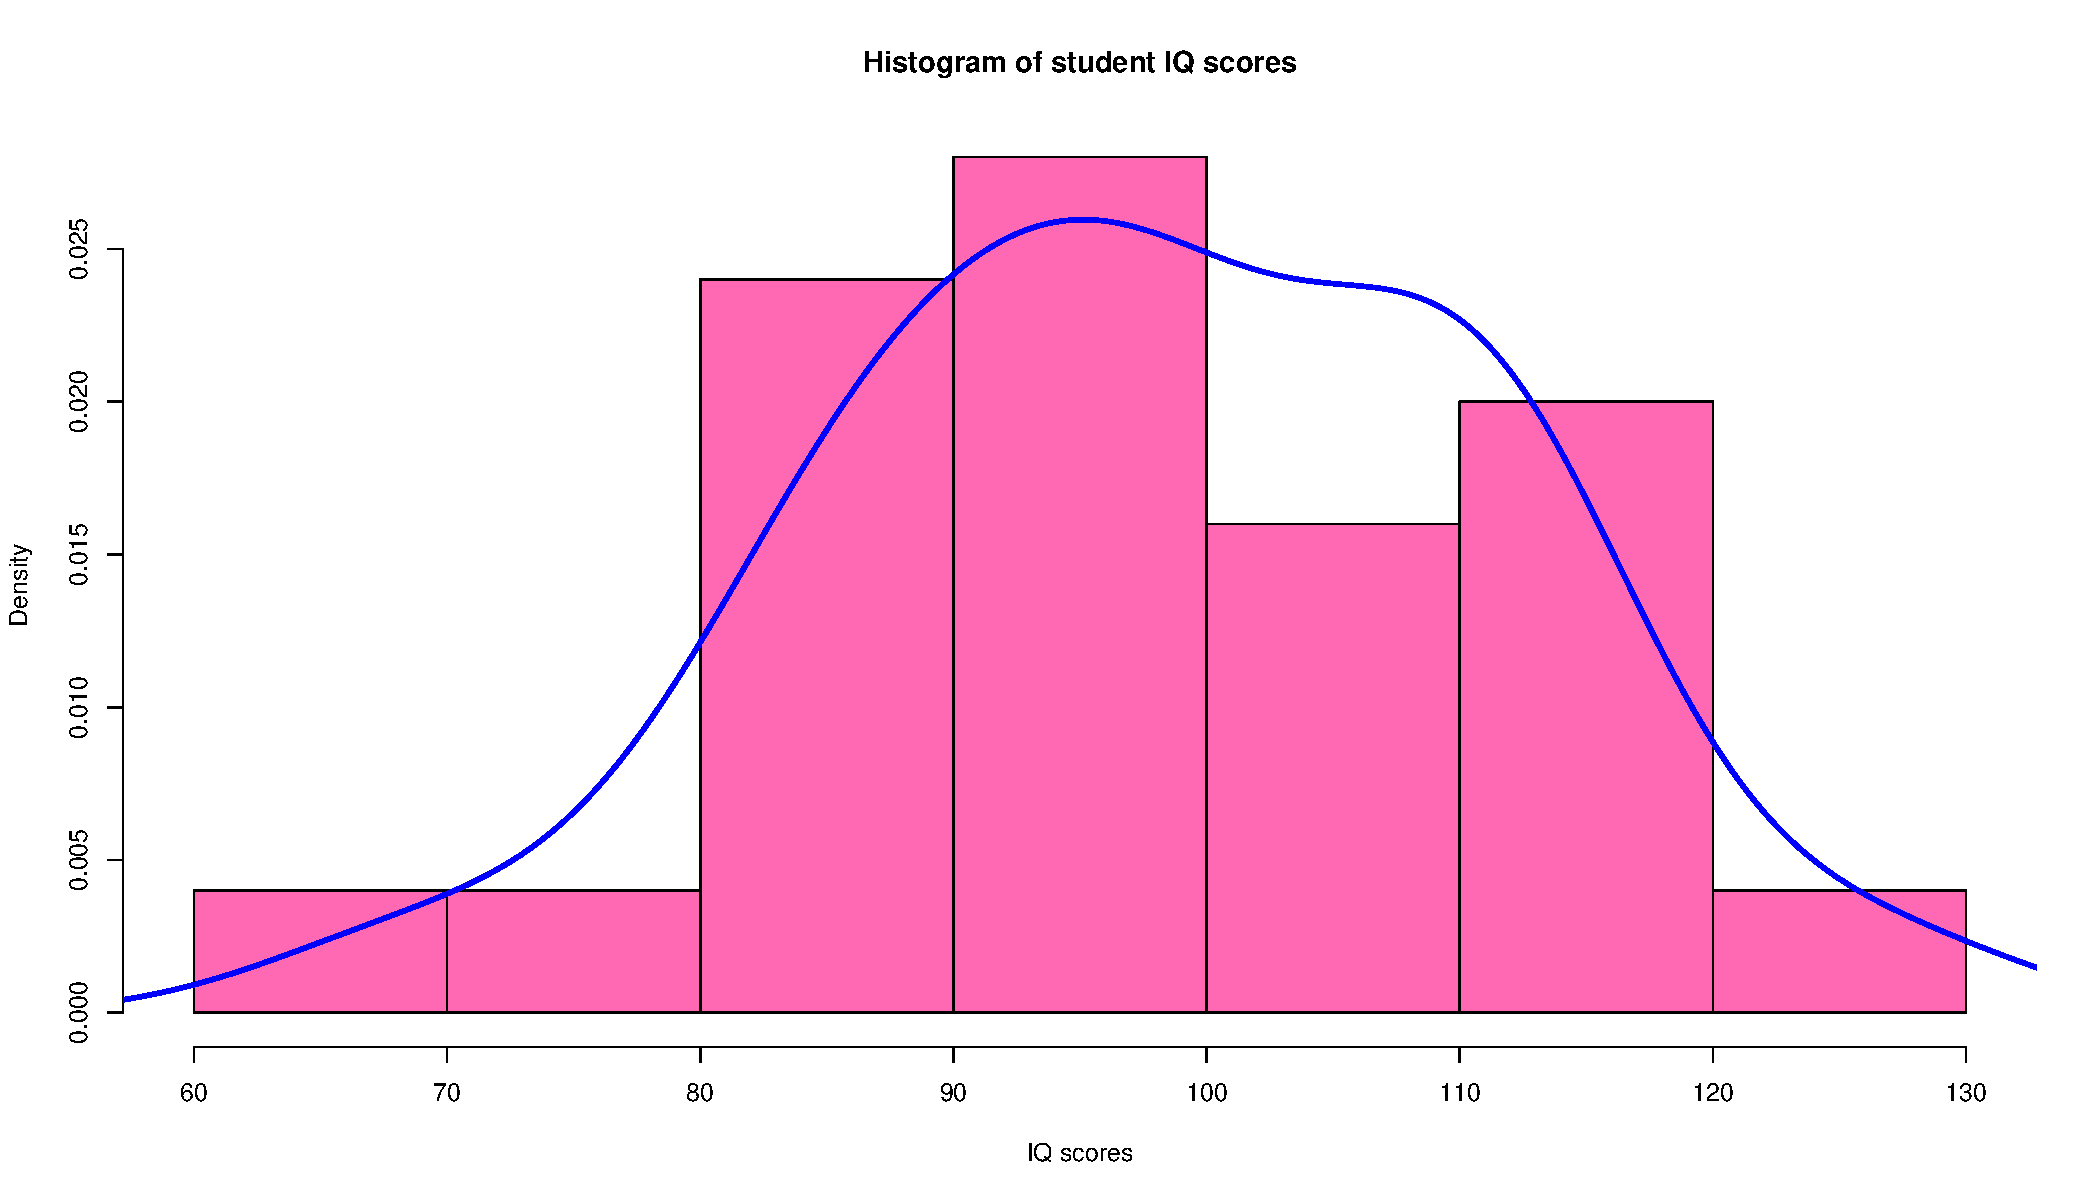
\includegraphics[width=0.95\linewidth]{IQ_histogram.pdf}
		\caption{Histogram showing the normal distribution of dataset "y"}
	\end{figure}
	
	Next, I found the critical value using the \texttt{qt()} function, and calculated a value of 1.71 (3 s.f.). Using the formula for the confidence interval stated above, I multiplied the t-critical value by the standard error and subtracted this value from the sample mean for the lower tail, and added to the sample mean for the upper tail.
	
	\lstinputlisting[language=R, firstline= 67,lastline=77]{PS01_Solutions_AV.R}
	
	The lower tail was a value of 93.96 (2 d.p.) and the upper tail was a value of 102.92 (2 d.p.). Therefore, the confidence interval at 90\% for the average student IQ at the school is [93.96, 102.92].
	
	\item \textbf{Next, the school counselor was curious  whether  the average student IQ in her school is higher than the average IQ score (100) among all the schools in the country.}\\ 
	
	\noindent \textbf{Using the same sample, conduct the appropriate hypothesis test with $\alpha=0.05$.}
	\vspace{0cm}
	
	To determine whether the average student IQ at the school is higher than the average IQ score among all schools in the country, I used a one-tailed signficance test. IQ is a quantitative variable and observations are assumed to be independent. Furthermore, the 25 students were randomly sampled.
	
	The null hypothesis predicts that the average IQ of the students is the same as or lower than the average IQ score of schools in the country, $\mu \le 100$. The alternative hypothesis predicts that the average IQ is higher than the average IQ score of schools in the country, $\mu > 100$.
	
	To calculate the t-score I used the formula: (sample mean - population mean) / standard error (SE). I used the sample mean (98.44) and standard error (2.62) calculated in Question 1, and the population mean (100) provided in Question 2. If the t-score is greater than the t-critical value then I reject the null hypothesis, as it is signficantly unlikely that any difference observed between the different IQ score averages is random or coincidental. If, on the other hand, the t-score is less than the t-critical value, then I fail to reject the null hypothesis. Failing to reject the null hypothesis means that there is not enough evidence to prove that the observed difference is not random.
	
	\lstinputlisting[language=R, firstline= 83,lastline=92]{PS01_Solutions_AV.R}
	
	I calculated the p-value to be 0.722 (3 s.f.), which is higher than the alpha value of 0.05. As $0.722 > 0.05$, I fail to reject the null hypothesis, which means that the test results are not statistically signficant. This indicates that there is insufficient evidence to prove that the average student IQ at the school is higher than the average IQ score of all schools in the country.
	
\end{enumerate}

\newpage

	\section*{Question 2: Political Economy}

\noindent \textbf{Researchers are curious about what affects the amount of money communities spend on addressing homelessness. The following variables constitute our data set about social welfare expenditures in the USA. }\\
\vspace{.5cm}


\begin{tabular}{r|l}
	\texttt{State} &\emph{50 states in US} \\
	\texttt{Y} & \emph{per capita expenditure on shelters/housing assistance in state}\\
	\texttt{X1} &\emph{per capita personal income in state} \\
	\texttt{X2} &  \emph{Number of residents per 100,000 that are "financially insecure" in state}\\
	\texttt{X3} &  \emph{Number of people per thousand residing in urban areas in state} \\
	\texttt{Region} &  \emph{1=Northeast, 2= North Central, 3= South, 4=West} \\
\end{tabular}

\vspace{.5cm}
\noindent \textbf{Explore the \texttt{expenditure} data set and import data into \texttt{R}.}
\vspace{.5cm}
\lstinputlisting[language=R, firstline=100, lastline=100]{PS01_Solutions_AV.R}  
\vspace{0cm}
\begin{itemize}

\item
\textbf{Please plot the relationships among \emph{Y}, \emph{X1}, \emph{X2}, and \emph{X3}? What are the correlations among them (you just need to describe the graph and the relationships among them)?}
\vspace{0cm}

To plot the relationships among Y, X1, X2, and X3, I first converted Region into a factor because it is a cateogrical variable, not a numerical quantity.

\lstinputlisting[language=R, firstline=107,lastline=111]{PS01_Solutions_AV.R}

I used \texttt{par} to create a 2 by 3 grid of six scatterplots showing the relationships between Y, X1, X2, and X3. I also chose to use a nested \texttt{for} loop inside a \texttt{for} loop in order to make my code neater and run more efficiently. Without a \texttt{for}, I would have had to copy and plot the code separately six times, which would have been time inefficient and could have lead to more manual errors. Nesting \texttt{for} loops is appropraite here because the code framework for each scatterplot is the same - only the variables (and thus x and y labels) differ. Using a nested \texttt{for} loop allowed me to pair each variable with another variable, creating six unique pairs.

\lstinputlisting[language=R, firstline= 127,lastline=161]{PS01_Solutions_AV.R}

Using a scatterplot graph seems appropriate in this case because all the variables are continuous numeric variables: expenditure, income, financial insecurity, and urban residents. Furthermore, a scatterplot provides an accurate visual representation of the relationship betweene each variable, allowing me to see (1) direction of the line of best fit; (2) how tightly clustered the data points are/any visual trend; (3) any outliers.

Figure 2 below shows the six scatterplot graphs. All six plots demonstrate a positive linear relationship between each pair of variables. Several outliers can be identified throughout each plot, however, and some plots in particular (such as Plots 4 and 6) show great variability and thus weaker correlations. At the top of each plot is the Pearson correlation coefficient (r), which measures both the strength and direction of a linear relationship between two continuous variables. These r-values fall into a range of $-1 \le r \le 1$, where a positive r-value indicates a positive correlation - that is, as one variable increases, the other variable tends to increase - and a negative r-value indicates a negative correlation - that is, as one variable increases, the other variable tends to decrease.

\begin{figure}[H]
	\centering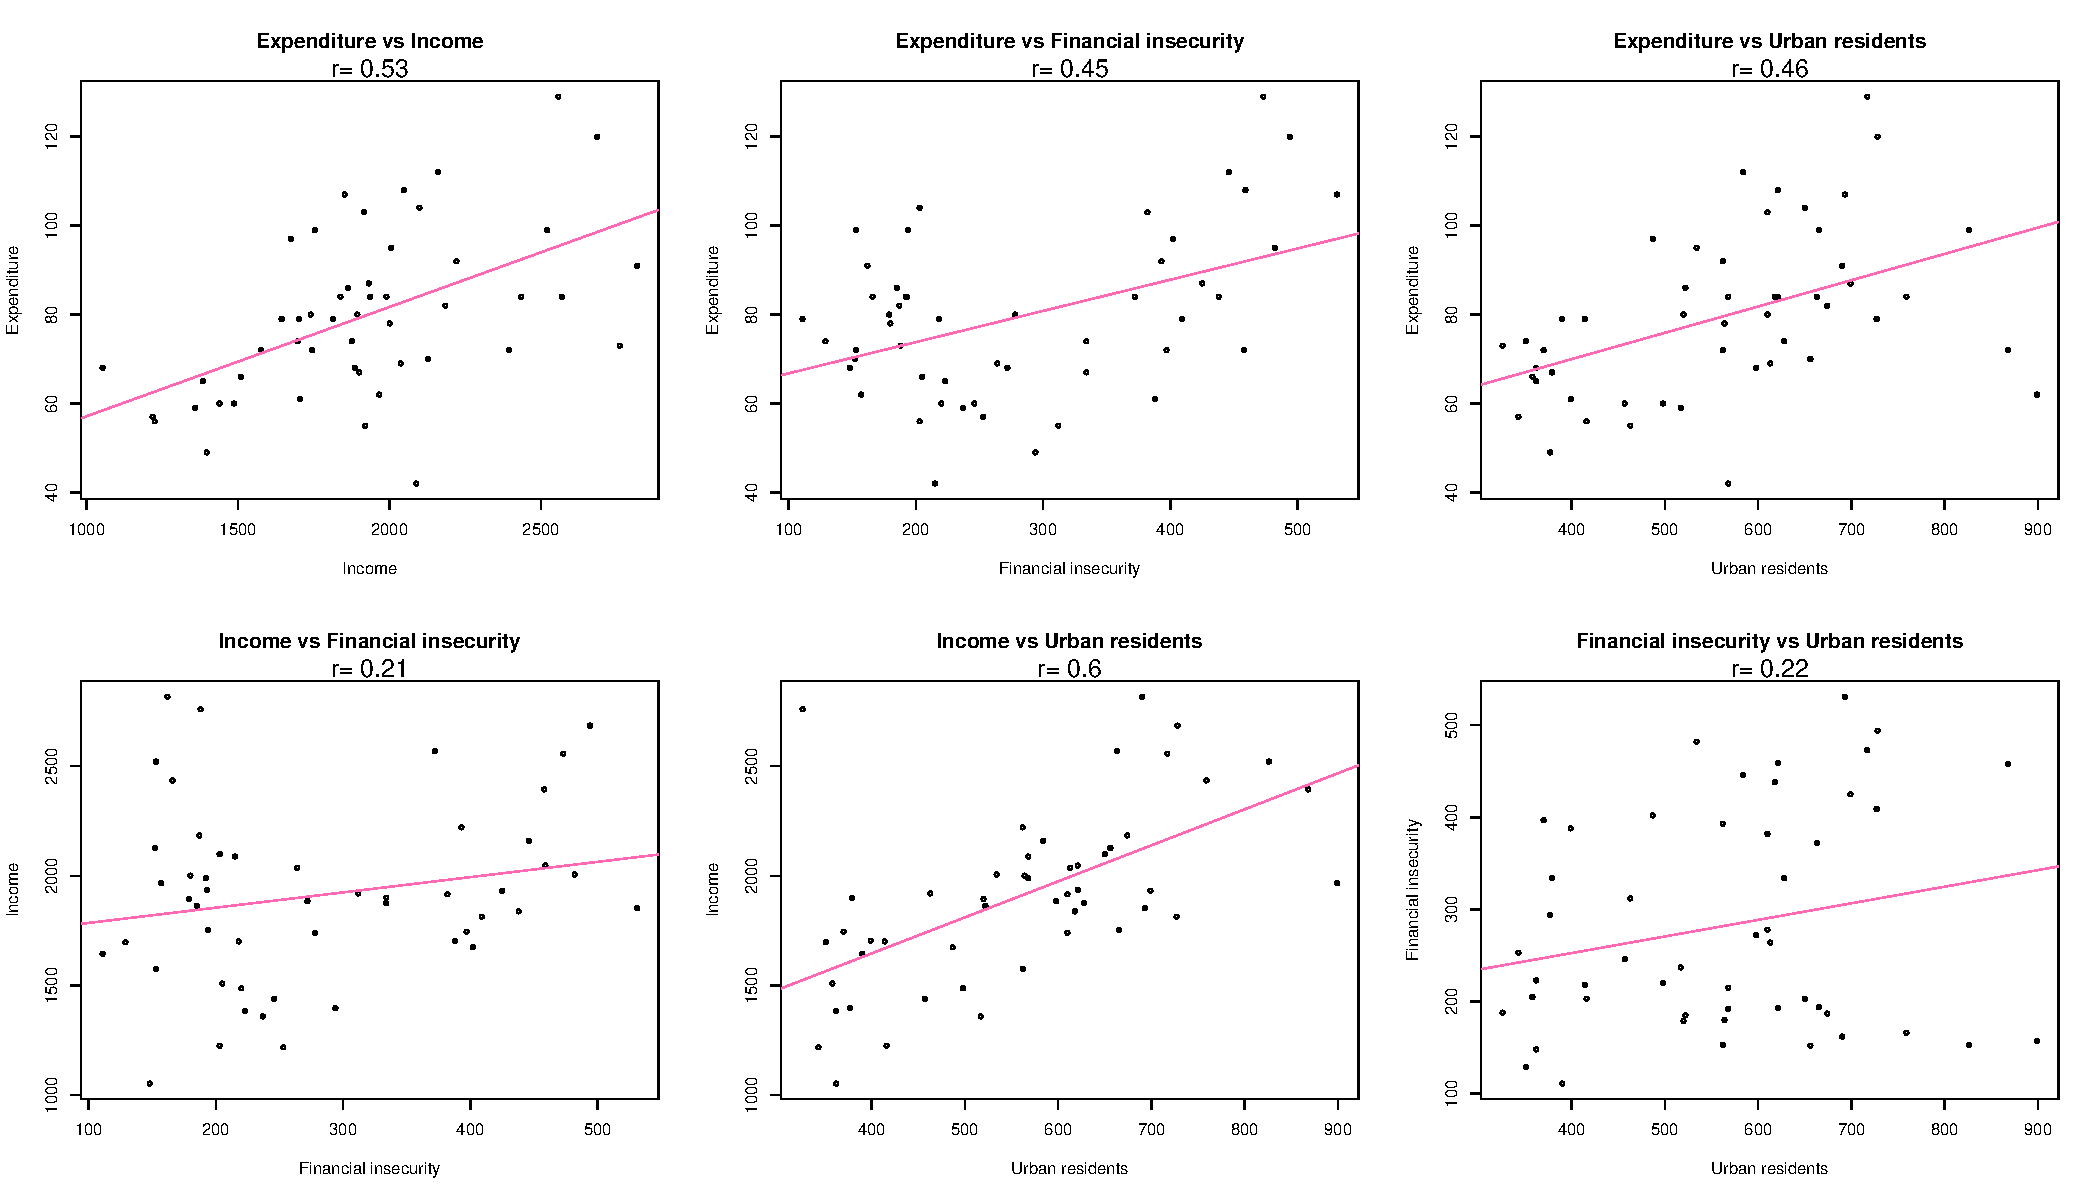
\includegraphics[width=0.95\linewidth]{P1_expenditure_relationships.pdf}
	\caption{Six scatterplots showing the relationships among expenditure, income, financial insecurity, and urban residents}
	\end{figure}

\textbf{Plot 1: "Expenditure vs Income"}
This plot shows the relationship between the per capita expenditure on shelters/housing assistance in a state and the per capita personal income in a state. There appears to be a moderately strong positive linear correlation, where r =0.53. This indicates that states with higher per capita personal income spend more on housing and shelters than states with lower per capita personal incomes.
\vspace{0.5cm}

\textbf{Plot 2: "Expenditure vs Financial insecurity"}
This shows the per capita expenditure on shelters/housing assistance in a state and the number of residents per 100,000 that are "financially insecure" in a state. It shows a moderately strong positive linear correlation, where r=0.45. The data points are less tightly clustered as in the first plot but there still appears to be an upward trend, indicating that when the state's residents are more financially insecure, there is higher spending on shelters and housing assistance.
\vspace{0.5cm}

\textbf{Plot 3: "Expenditure vs Urban residents"}
This shows the per capita expenditure on shelters/housing assistance in a state and the number of people per thousand residing in urban areas in a state. It shows a moderately strong positive linear correlation, where r=0.46. This means that the more urban residents there are, the higher the expenditure on shelters/housing assistance is in a given state.
\vspace{0.5cm}

\textbf{Plot 4: "Income vs Financial insecurity"}
This shows the per capita personal income in a state and the number of residents per 100,000 that are "financially insecure" in a state. There is a very weak positive correlation, where r=0.21. Indeed, this is the weakest correlation of all six scatterplots. This indicates that in states where financial insecurity is higher, personal income tends to be higher, too.
\vspace{0.5cm}

\textbf{Plot 5: "Income vs Urban residents"}
This plot shows the per capita personal income in a state and the number of people per thousand residing in urban areas in a state. There is a strong positive linear correlation, where r=0.6. Indeed, this is the strongest correlation of all six scatterplots. This indicates that with more urban residents per thousand in a state, the higher the personal income in a state tends to be.
\vspace{0.5cm}

\textbf{Plot 6: "Financial insecurity vs Urban residents"}
This plot shows the number of residents per 100,000 that are "financially insecure" in a state and the number of of people per thousand residing in urban areas in a state. There is a very weak positive correlation, where r=0.22. This indicates that with more urban residents per thousand in a state, financial insecurity tends to be higher.
\vspace{0.5 cm}

\item
\textbf{Please plot the relationship between \emph{Y} and \emph{Region}? On average, which region has the highest per capita expenditure on housing assistance?}
\vspace{0cm}

I used a boxplot to show the relationship between Y and Region because Region is a categorical variable, rather than numerical. This way, I am able to show the per capita expenditure on shelter/housing assistance as per each Region in the US.

\lstinputlisting[language=R, firstline= 179,lastline=198]{PS01_Solutions_AV.R}

Mean and median are good indicators of which region has the highest expenditure because they both measure the "middle" of the data, in complementary ways. The median is the middle value of the data and resistant to outliers, meaning that it is an accurate representative of a dataset. The mean, on the other hand, is highly sensitive to outliers and includes every data point, making it a good representative of the dataset. For these reasons, a boxplot provides a more descriptive visual of which region has highest per capita expenditure.

I used the code below to more precisely gauge the mean and median values. I found that the mean expenditure on housing assistance in the Northeast, North Central, South, and West regions are 79.4, 83.9, 69.2, and 88.3, respectively (all rounded to 3 s.f.). Similarly, the median expenditure on housing assistance in these regions are 72, 83, 67, and 87, respectively. This is displayed in Table 1. Both mean and median show that the West region has highest per capita expenditure on housing assistance.

\lstinputlisting[language=R, firstline= 202,lastline=227]{PS01_Solutions_AV.R}


% Table created by stargazer v.5.2.3 by Marek Hlavac, Social Policy Institute. E-mail: marek.hlavac at gmail.com
% Date and time: Thu, Oct 08, 2026 - 14:37:47
\begin{table}[!htbp] \centering 
  \caption{Mean and median expenditure by Region} 
  \label{tab:region_mean_median} 
\begin{tabular}{@{\extracolsep{5pt}} ccc} 
\\[-1.8ex]\hline 
\hline \\[-1.8ex] 
Region & Mean expenditure & Median expenditure \\ 
\hline \\[-1.8ex] 
North Central & $83.9$ & $83$ \\ 
Northeast & $79.4$ & $72$ \\ 
South & $69.2$ & $67$ \\ 
West & $88.3$ & $87$ \\ 
\hline \\[-1.8ex] 
\end{tabular} 
\end{table} 

\vspace{1.2 cm}

The idea that the West region has the highest expenditure is further supported by the boxplot in Figure 3, which shows the per capita expenditure in the Northeast, North Central, South, and West regions in the US. The boxplots are a good visual representation that the West region has the highest mean and median. Boxplots also display the inter-quartile range (IQR), showing where the middle 50\% of the data lie. Accordingly, the West region has the highest per capita expenditure on housing assistance.

\begin{figure}[H]
	\centering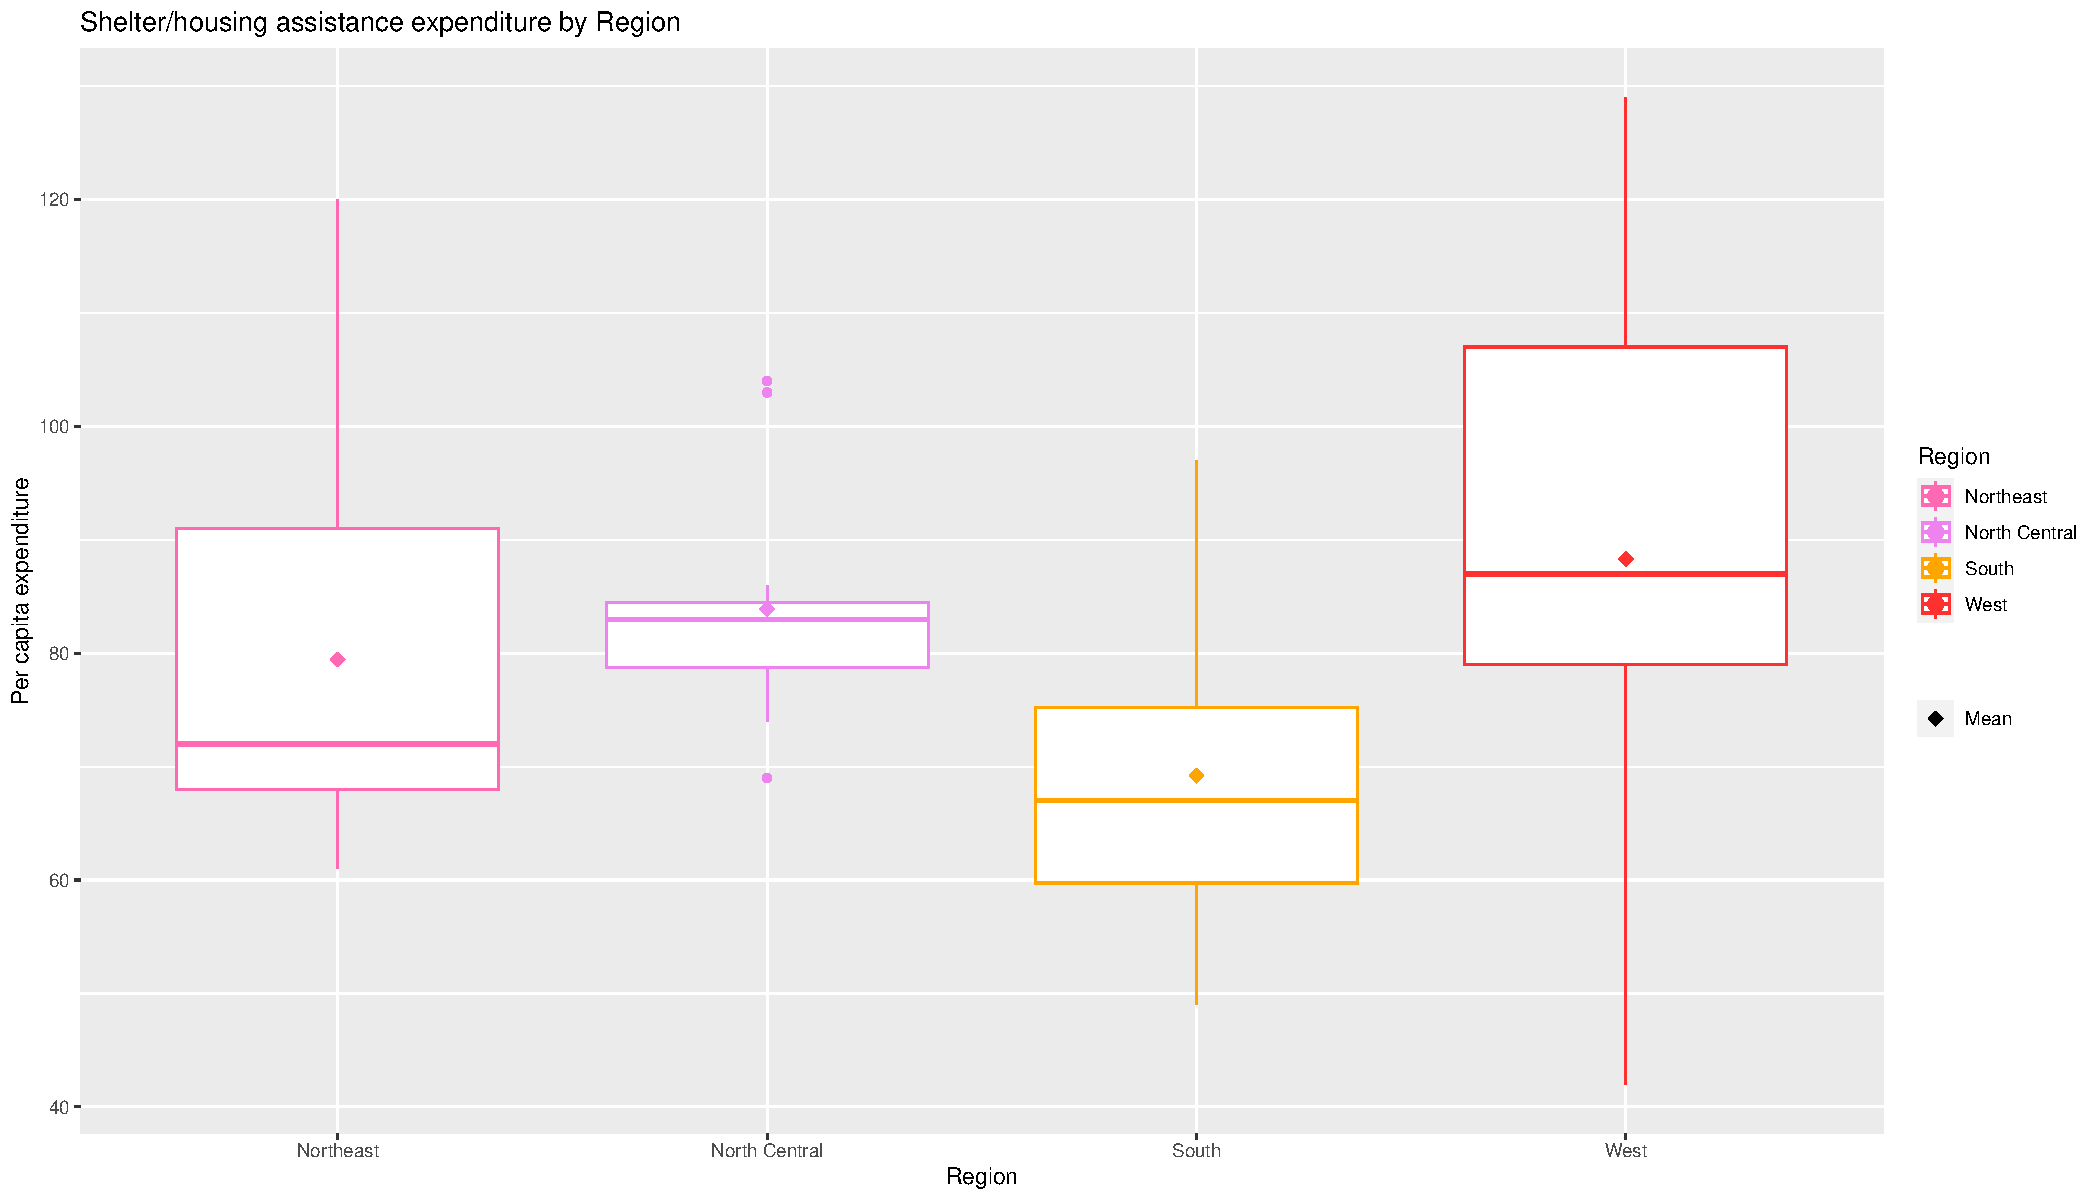
\includegraphics[width=0.95\linewidth]{P1_expenditure_relationship_region.pdf}
	\caption{Boxplot of expenditure on shelter/housing assistance colour-coded by Region }
\end{figure}

\item
\textbf{Please plot the relationship between \emph{Y} and \emph{X1}? Describe this graph and the relationship. Reproduce the above graph including one more variable \emph{Region} and display different regions with different types of symbols and colors.}
\end{itemize}

I used a scatterplot graph using \texttt{ggplot()} to plot the relationship between Y and X1 (per capita expenditure vs per capita personal income), similar to that in Figure 2.

\lstinputlisting[language=R, firstline= 234,lastline=245]{PS01_Solutions_AV.R}

Figure 3 shows a scatterplot of per capita personal income against per capita expenditure on shelter/housing assistance. It shows a strong positive correlation. Indeed, the Pearson correlation coefficient (r) (shown in Figure 2) is 0.53, which suggests a moderate correlation strength. The datapoints are moderately clustered around the line of best fit. This means that as per capita personal income increases, per capita expenditure tends to increase, too. However, there is still a fair amount of variability around the line of best fit.

\begin{figure}[H]
	\centering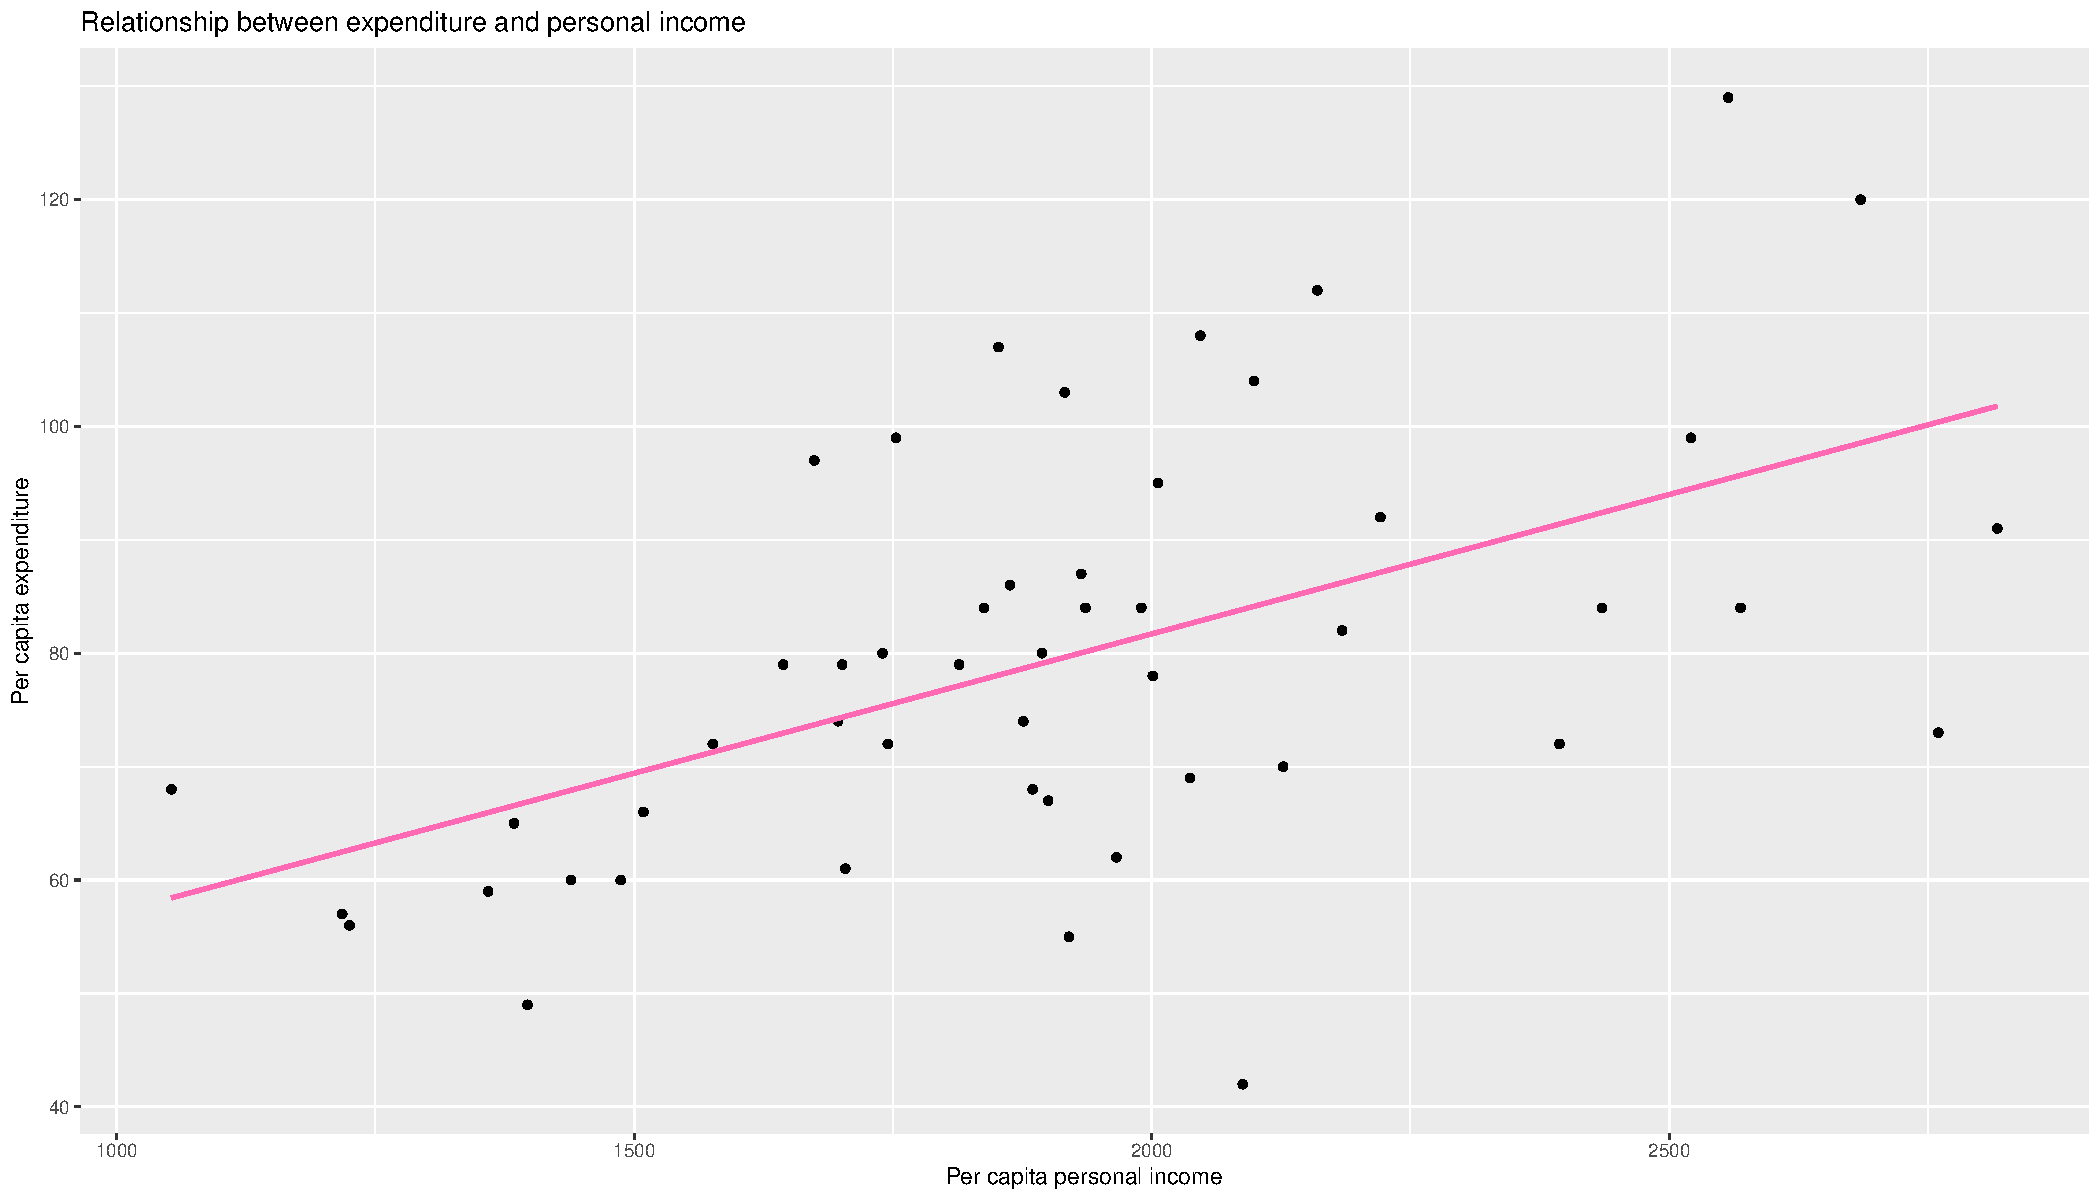
\includegraphics[width=0.95\linewidth]{P1_expenditure_income.pdf}
	\caption{Boxplot of expenditure on shelter/housing assistance colour-coded by Region }
\end{figure}

Next, I used \texttt{ggplot()} again to reproduce the graph in Figure 4 with the addition of a third variable: Region. I distinguished the different regions both by colour and by shape (as seen in the legend in Figure 5).

\lstinputlisting[language=R, firstline= 252,lastline=269]{PS01_Solutions_AV.R}

\begin{figure}[H]
	\centering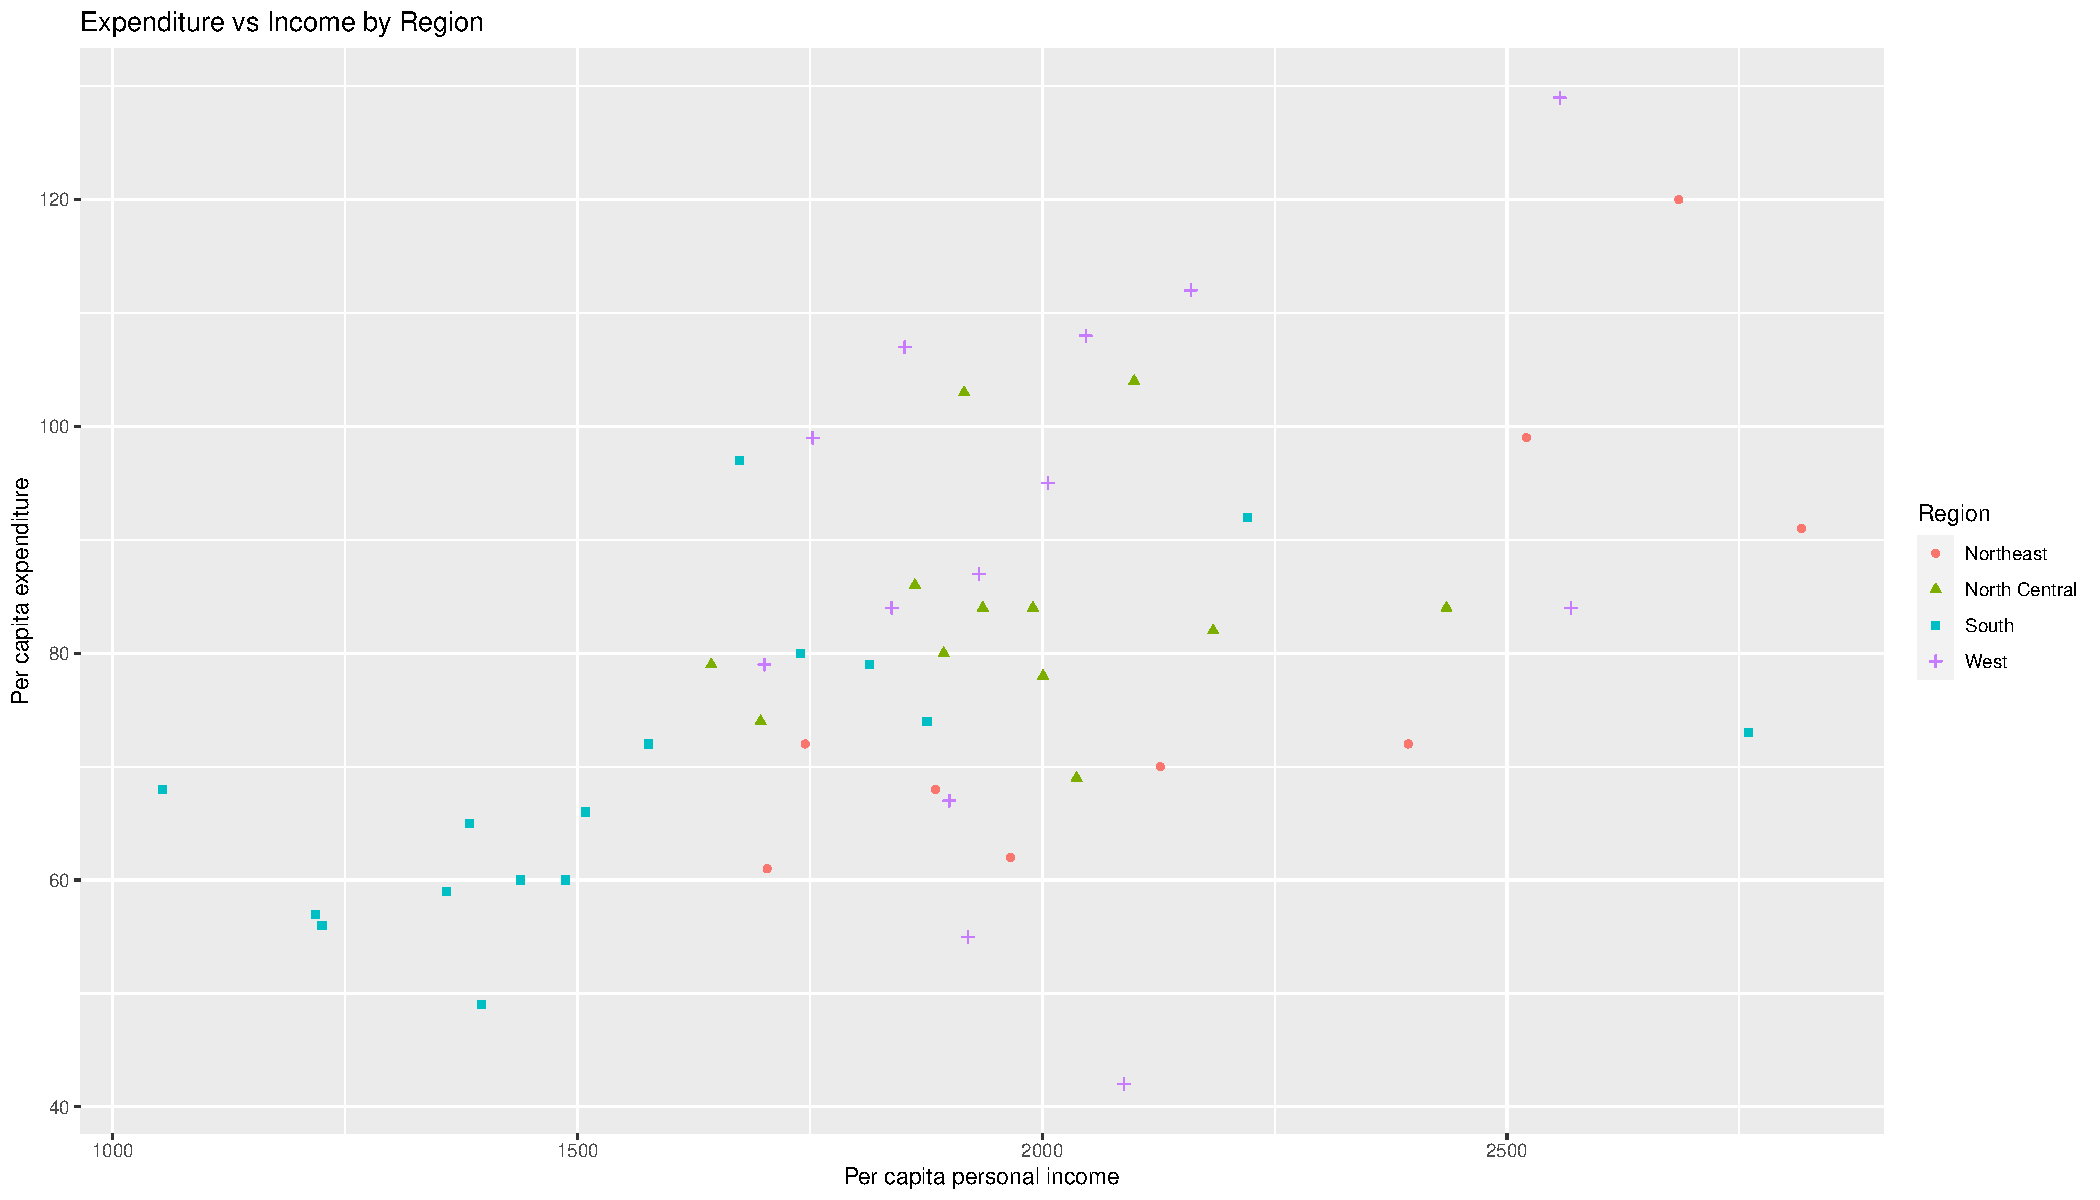
\includegraphics[width=0.95\linewidth]{P1_expenditure_income_region.pdf}
	\caption{Boxplot of expenditure on shelter/housing assistance colour-coded by Region }
\end{figure}

Figure 5 shows regional variation between per capita personal income and per capita expenditure. The scatterplot indicates that the South region tends to have lower per capita personal income and, by association, lower per capita expenditure. The Northeast and North Central regions display similar datapoints, generally clustered in the middle of the scatterplot. Lastly, the West region shows generally higher per capita personal income and, by association, higher per capita expenditure on shelter/housing assistance.

\end{document}
